\providecommand{\main}{..}
\documentclass[../COS3712_Notes.tex]{subfiles}

\begin{document}
  \setcounter{chapter}{5}
  \chapter{From Vertices to Fragments}
    \begin{sidenote}{Textbook}
      In the textbook, this section corresponds to Chapter 8: From Geometry to Pixels.
    \end{sidenote}

    \concept{Clipping} involves eliminating objects that lie outside the viewing volume,
    and thus cannot be visible in the image.
    \concept{Rasterization} produces fragments from the remaining objects.
    These fragments can contribute to the final image.
    \concept{Hidden-surface~removal} determines which fragments correspond to objects
    that are visible, namely, those that are in the view volume and are not blocked
    from view by other objects closer to the camera.

    \section{Basic Implementation Strategies}
      \begin{figure}
        \begin{center}
          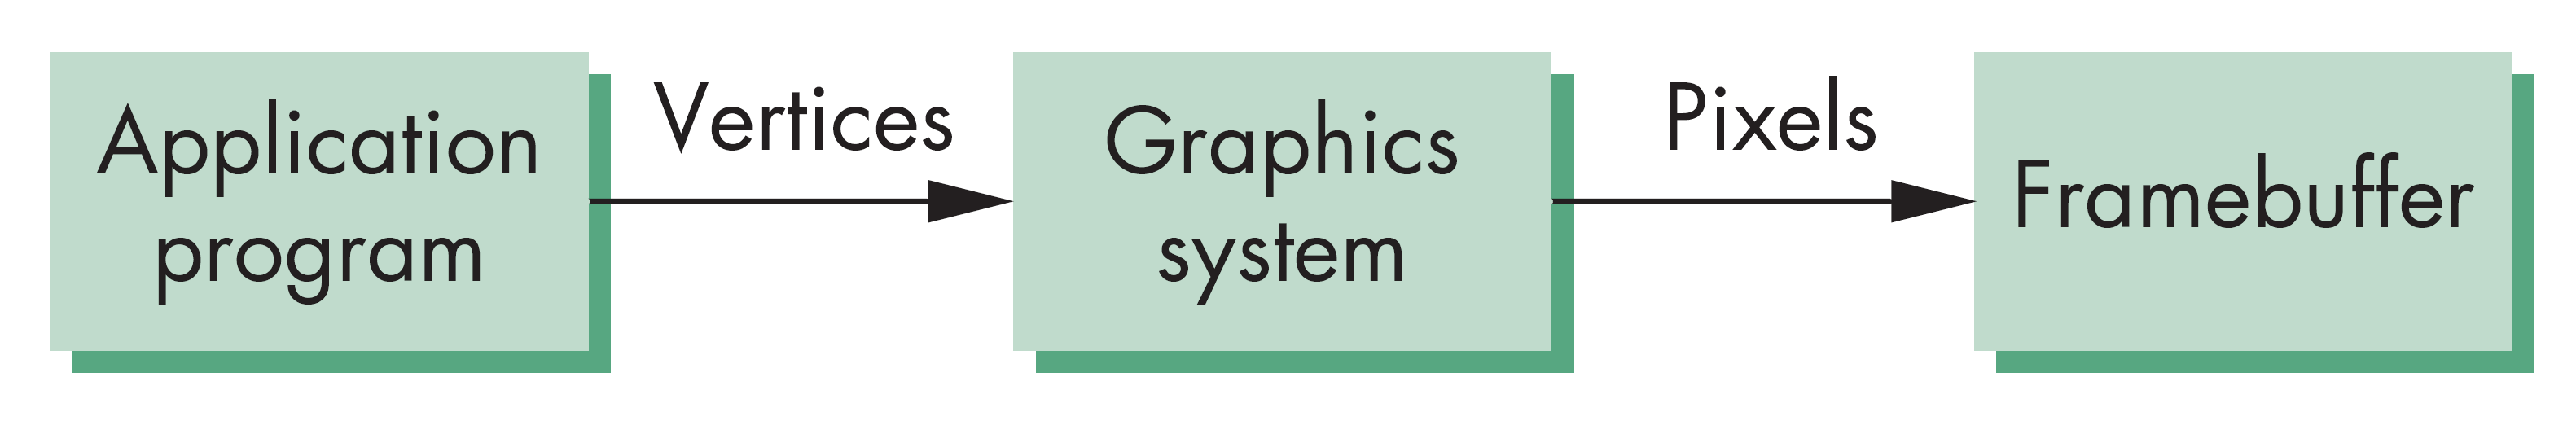
\includegraphics[width=0.7\textwidth]{\main/images/chapter06/graphics_process.png}
        \end{center}
        \caption{High-level view of the graphics process}
      \end{figure}

      In computer graphics, we start with an application program, and end with an image.
      We can consider this process as a black box whose inputs are the vertices and states
      defined in the program -- geometric objects, attributes, camera specifications --
      and whose output is an array of coloured pixels in the framebuffer.

      Within the black box, we must perform many tasks, including transformations,
      clipping, shading, hidden-surface removal, and rasterization of the primitives
      that can appear on the display.
      These tasks can be organised in a variety of ways, but regardless of the strategy
      we adopt, we must always do two things:
      \begin{enumerate}[nosep]
        \item We must pass every geometric object through the system, and
        \item we must assign a colour to every pixel in the colour buffer that is displayed.
      \end{enumerate}

      Suppose we think of what goes into the black box in terms of a single program
      that carries out the entire process.
      Because this program must assign a value to every pixel and must process every
      geometric primitive (and light source),
      we expect this program to contain at least two loops that iterate over these basic
      variables.
      The variable we choose to control the outer loop determines the flow of the entire
      implementation process.
      There are two fundamental strategies: the \concept{image-oriented} approach, and the
      \concept{object-oriented} approach.

      \begin{definition}{Object Oriented Approach}
        The outer loop iterates over the objects.

        A pipeline renderer fits this description.
        Vertices are defined by the program and flow through a sequence of modules that
        transforms them, colours them, and determines whether they are visible.

        After a polygon passes through geometric processing, the rasterization
        of this polygon can potentially affect any pixels in the framebuffer.

        Most implementations that follow this approach are based on construction of a
        rendering pipeline containing hardware or software modules for each of the tasks.
        Data (vertices) flow \emph{forward} through the system.

        In the past, the major limitations of the object-oriented approach were the
        large amount of memory required and the high cost of processing each object
        independently.
        Any geometric primitive that emerges from the geometric processing can potentially
        affect any set of pixels in the framebuffer.
        So, the entire colour buffer, and various other buffers, must be of the size of the
        display, and must be available at all times.

        Today, the main limitation of object-oriented implementations is that they cannot
        handle most global calculations.
        Because each geometric primitive is processed independently
        -- and in an arbitrary order --
        complex shading effects that involve multiple geometric objects,
        such as reflections,
        cannot be handled except by approximate methods.
        The major exception is hidden-surface removal, where the $z$-buffer is used to store
        global information.
      \end{definition}

      \begin{definition}{Image-Oriented Approach}
        The outer loop iterates over pixels, or rows of pixels called \concept{scan~lines},
        that constitute the framebuffer.

        For each pixel, we work \emph{backward}, trying to determine which geometric primitives
        can contribute to its colour.

        The advantages of this approach are that we need only limited display memory
        at any time and that we can hope to generate pixels
        at the rate and in the order required to refresh the display.
        Because the results of most calculations do not differ from pixel to pixel
        (or scan line to scan line),
        we can use this coherence in our algorithms by developing incremental forms
        for many of the steps in the implementation.

        The main disadvantage of this approach is that, unless we first build a data structure
        from the geometric data, we do not know which primitives affect which pixels.
        Such a data structure can be complex, and may imply that all the geometric data
        must be available at all times during the rendering process.
        For problems with very large databases, even having a good data representation
        may not avoid memory leaks.
        However, because image-space algorithms have access to all objects for each pixel,
        they are well suited to handle global effects, such as shadows and reflections.
      \end{definition}

      Within these two major categories specified by two loops, each may contain other loops.

    \section{Four Major Tasks}
      There are four major tasks that any graphics system must perform to render a geometric
      entity, as that entity passes from definition in a user program to possible display
      on an output device:
      \begin{enumerate}[nosep]
        \item Modelling
        \item Geometry processing
        \item Rasterization
        \item Fragment processing
      \end{enumerate}

      \begin{definition}{Modelling}
        The usual results of the modelling process are sets of vertices that specify
        a group of geometric objects supported by the rest of the system.
        We can look at the modeller as a black box that produces geometric objects
        and is usually a user program.

        There are other tasks a modeller might perform, such as clipping.
        A user can generate geometric objects in their program,
        and hope that the rest of the system can process these objects at the rate at which
        they are produced, or the modeller can attempt to ease the burden on the rest of the
        system by minimising the number of objects that it passes on.
        The latter approach often means that the modeller may do some of the same jobs
        as the result of the system, albeit with different algorithms.
        In the case of clipping, the modeller knows more about the specifics of the application,
        and can often use a good heuristic to eliminate many, if not most,
        primitives before they are sent on through the standard viewing process.
      \end{definition}

      \begin{definition}{Geometry Processing}
        Geometry processing works with vertices.
        The goals of the geometry processor are to determine which geometric objects
        appear on the display, and to assign shades or colours to the vertices of these objects.
        Four processes are required:
        \begin{enumerate}[nosep]
          \item Projection
          \item Primitive Assembly
          \item Clipping
          \item Shading
        \end{enumerate}

        Usually, the first step in geometry processing is to change representations
        from object coordinates to camera coordinates using the model-view transformation.
        The second step is to transform vertices using the projection transformation
        to a normalised view volume in which objects that might be visible are contained
        in a cube centred at the origin.
        Vertices are now represented in clip coordinates.

        Before clipping can take place, vertices must be grouped into objects,
        a process known as \concept{primitive assembly}.
        When vertices reach the rasterizer, they can no longer
        be processed individually, but only as primitives.

        After clipping takes place, the remaining vertices are still in four-dimensional
        homogeneous coordinates.
        Perspective division converts theme to 3D representations in normalised device coordinates.
        Per-vertex shading is also performed during this stage.

        Collectively, these operations constitute \concept{front-end~processing}.
        All are carried out on a vertex-by-vertex basis.
      \end{definition}

      \begin{definition}{Rasterization (Scan Conversion)}
        We need to retain depth information for hidden-surface removal.
        But only the $x, y$ values of the vertices are needed to determine which pixels
        in the framebuffer can be affected by the primitive.
        To generate a set of fragments that give the locations of the pixels in the framebuffer
        corresponding to these vertices, we only need their $x, y$ components,
        or, equivalently, the results of the orthogonal projection of these vertices.
        We determine these fragments through a process called \concept{rasterization}
        or \concept{scan~conversion}.
        For line segments, rasterization determines which fragments should be used to approximate
        a line segment between the projected vertices.
        For polygons, rasterization determines which pixels lie inside the 2D polygon
        determined by the projected vertices.

        The colours we assign to these fragments can be determined by the vertex attributes,
        or obtained by interpolating the shades at the vertices that are computed.
        Objects more complex than line segments and polygons are usually approximated
        by multiple line segments and triangles.

        The rasterizer starts with vertices in normalised device coordinates,
        but outputs fragments whose location are in units of the display
        -- \concept{window coordinates}.
        The projection of the clipping volume must appear in the assigned viewport.
        We use the term \concept{screen~coordinates} to refer to the 2D system that is the same
        as the window coordinates, but lacks the depth coordinate.
      \end{definition}

      \begin{definition}{Fragment Processing}
        In the simplest situations, each fragment is assigned a colour by the rasterizer,
        and this colour is placed in the framebuffer at the locations corresponding to the
        fragment's location.

        Per-fragment shading, texture-mapping, bump-mapping, alpha blending,
        antialiasing, and hidden-surface removal all take place in this stage.
      \end{definition}

    \section{Clipping}
      \begin{definition}{Clipping}
        The process of determining which primitives, or parts of primitives,
        fit within the clipping or view volume defined by the application program.
      \end{definition}

      Clipping is done before the perspective division that is necessary if the $w$-component
      of a clipped vertex is not equal to 1.
      The portions of all primitives that can possibly be displayed lie within the cube
      \begin{align*}
        w \geq x \geq -w \\
        w \geq y \geq -w \\
        w \geq z \geq -w
      \end{align*}
      This coordinate system is called \concept{normalised device coordinates}
      because it depends on neither the original application units nor the particulars
      of the display device,
      although the information to produce the correct image is retained in this coordinate system.
      The projection has also only been carried out partially: we still need to do the
      perspective division and the final orthographic projection.

    \section{Line-Segment Clipping}
      A \concept{clipper} determines which primitives, or parts of primitives,
      can possibly appear on the display and be passed on the rasterizer.
      Primitives that fit within the specified view volume pass through the clipper,
      or are \concept{accepted}.
      Primitives that cannot appear on the display are \concept{rejected} or \concept{culled}.
      Primitives that are only partially within the view volume must be clipped such that
      any part lying outside the volume is removed.

      \subsection{Cohen-Sutherland Clipping}
        We want to avoid intersection calculations with the sides of the window,
        because each intersection calculation requires a floating point division.
        The \concept{Cohen-Sutherland algorithm} replaces most of the expensive floating
        point multiplications and divisions with a combination of floating point subtractions
        and bit operations.

        The algorithm starts by extending the sides of the window to infinity,
        thus breaking up space into nine regions:
        \begin{center}
          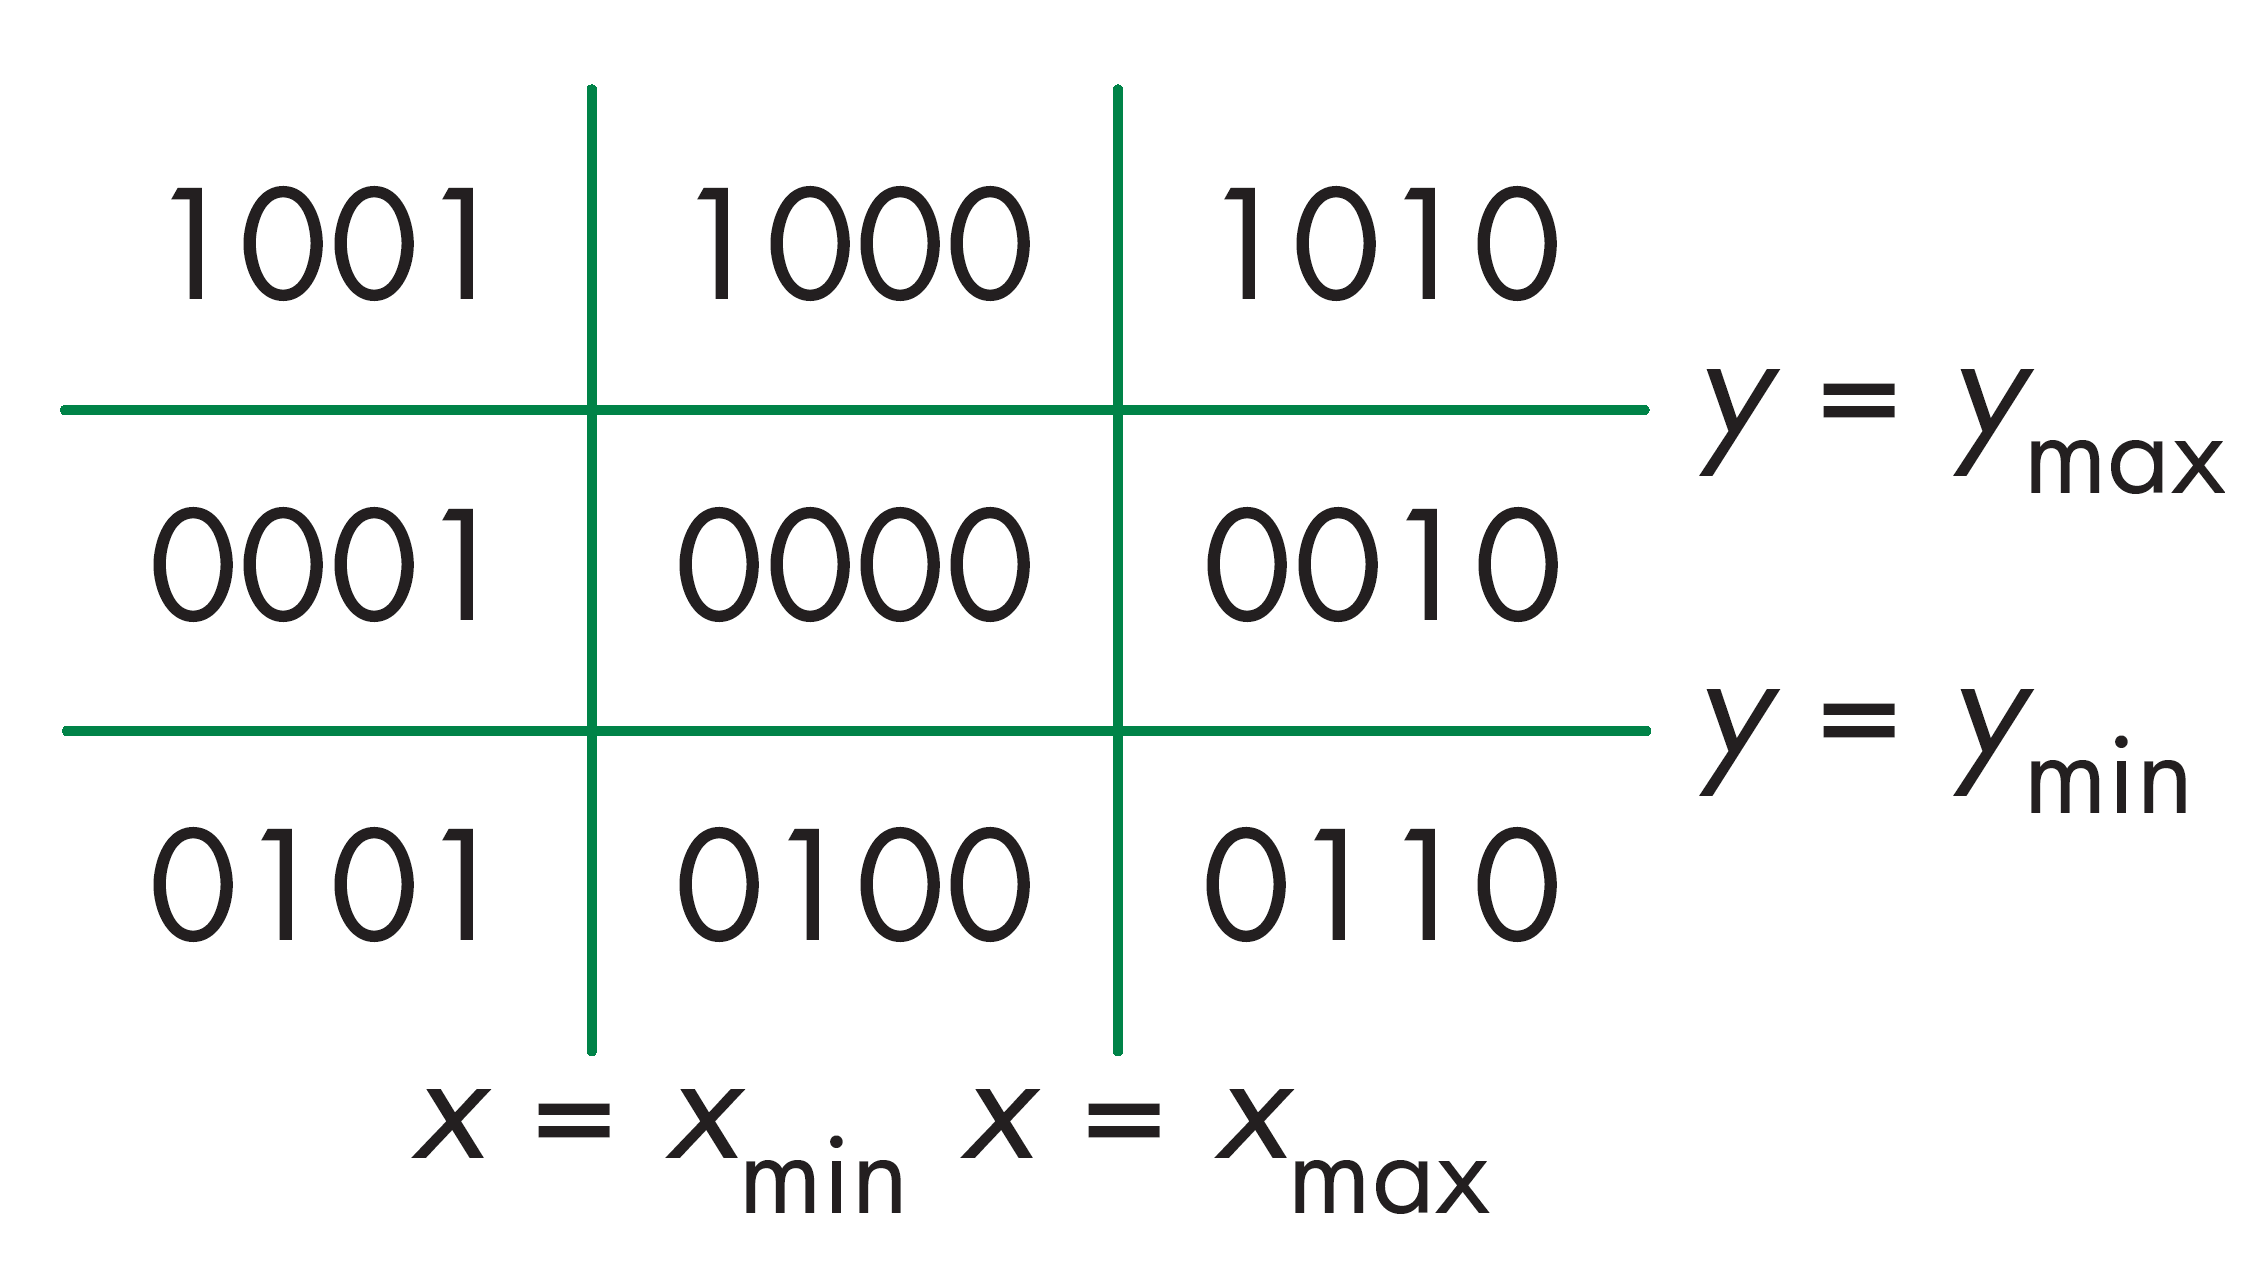
\includegraphics[height=4cm]{\main/images/chapter06/cohen_sutherland.png}
        \end{center}
        Each region can be assigned a unique 4-bit binary number, or \concept{outcode}, $b_0 b_1 b_2 b_3$
        as follows.
        Suppose that $(x, y)$ is a point in the region; then
        \begin{align*}
          b_0 = \begin{cases}
            1 \quad \text{if } y > y_{\text{max}}\\
            0 \quad \text{otherwise.}
          \end{cases}
        \end{align*}
        Likewise, $b_1$ is 1 if $y < y_{\text{min}}$, and $b_2$ and $b_3$ are determined similarly,
        but for $x$.
        For each endpoint of a line segment, we first compute the endpoint's outcode,
        a step that can require eight floating-point subtractions per line segment.

        \begin{figure}[b]
          \begin{center}
            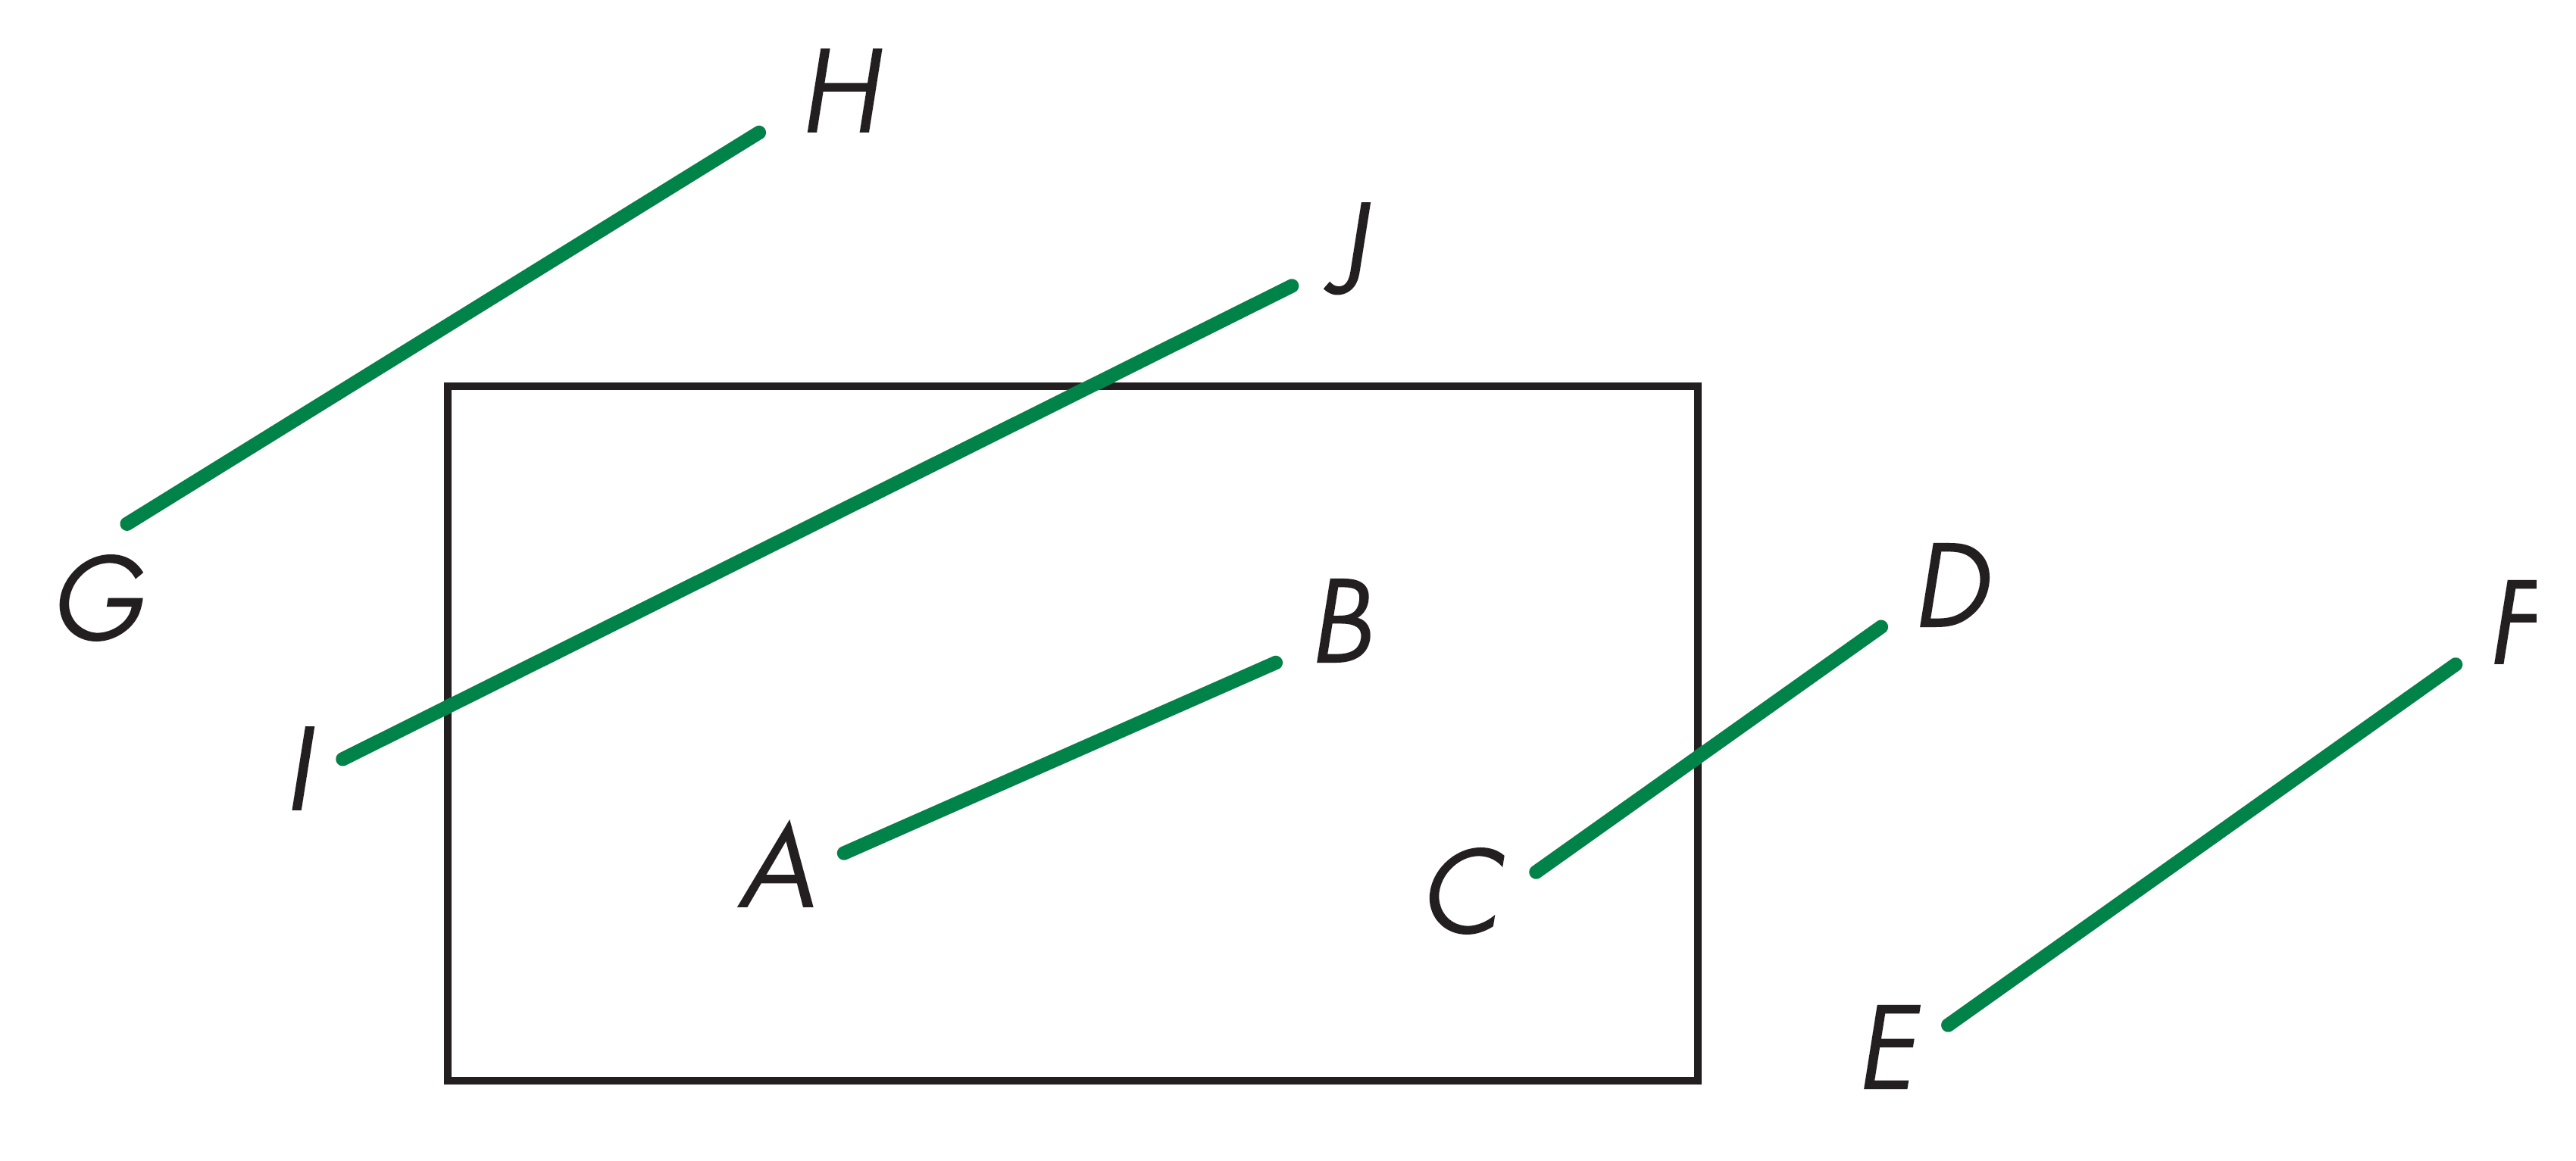
\includegraphics[width=0.7\textwidth]{images/chapter06/outcode_cases.png}
          \end{center}
          \caption{Cases of outcodes in Cohen-Sutherland algorithm.}
          \label{fig:cases}
        \end{figure}

        Consider a line segment whose outcodes are given by $o_1 = \text{outcode}(x_1, y_1)$ and
        $o_2 = \text{outcode}(x_2, y_2)$.
        We can now reason on the basis of these outcodes.
        There are four cases:
        \begin{enumerate}
          \item $(o_1 = o_2 = 0)$. Both endpoints are inside the clipping window,
            as is true for the segment~$AB$ in \autoref{fig:cases}.
            The entire line segment is inside, and the segment can be sent on to be rasterized.
          \item ($o_1 \neq 0, o_2 = 0$; or vice versa). One endpoint is inside the clipping window;
            one is outside, as in segment~$CD$ in \autoref{fig:cases}.
            The line segment must be shortened.
            The nonzero outcode indicates which edge or edges of the window are crossed
            by the segment.
            One or two intersections must be computed.
            After one segment is computed, we can compute the outcode of the point of intersection
            to determine whether another intersection calculation is required.
          \item ($o_1 \text{ \& } o_2 \neq 0$). Two endpoints lie on the same outside edge of the
            window, as in segment~$EF$ in \autoref{fig:cases}.
            Calculated by taking the bitwise \textsc{and} of the outcodes.
            The line segment can be discarded.
          \item ($o_1 \text{ \& } o_2 = 0$). Both edges are outside, but they are on the outside
            of different edges of the window.
            This is the case for segments~$GH$ and $IJ$ in \autoref{fig:cases}.
            We cannot tell from just the outcodes whether the segment can be discarded,
            or must be shortened.
            The best we can do is to intersect with one of the sides of the window and to check
            the outcode of the resulting point.
        \end{enumerate}

        With this algorithm, we do intersection calculations only when they are needed,
        as in the second case, or where the outcodes did not contain enough information,
        as in the fourth case.

        The Cohen-Sutherland algorithm works best when there are many line segments but few
        are actually displayed.
        In this case, most of the line segments lie fully outside one or two of the extended
        sides of the clipping rectangle and thus can be eliminated on the basis of their outcodes.
        The other advantage is that this algorithm can be extended to three dimensions.
        The main disadvantage of this algorithm is that it must be used recursively.

      \subsection{Liang-Barsky Clipping}
        If we use the parametric form for lines, we can approach the clipping of line segments
        in a more efficient manner.
        Suppose we have a line segment defined by the two endpoints
        $\mathbf{p}_1 = [x_1, y_1]^{T}$ and $\mathbf{p}_2 = [x_2, y_2]^{T}$.
        We can use these endpoints to define a unique line that we can express parametrically,
        either in matrix form:
        \begin{align*}
          \mathbf{p}(\mathbf{\alpha}) = (1 - \alpha)\mathbf{p}_1 + \alpha \mathbf{p}_2
        \end{align*}
        or as two scalar equations
        \begin{align*}
          x(\alpha) = (1 - \alpha)x_1 + \alpha x_2 \\
          y(\alpha) = (1 - \alpha)y_1 + \alpha y_2
        \end{align*}
        This form is robust and needs no changes for horizontal or vertical lines.
        As the parameter $\mathbf{\alpha}$ varies from 0 to 1, we move along the segment from
        $\mathbf{p}_1$ to $\mathbf{p}_2$.
        Negative values give points on the other side of $\mathbf{p}_1$ from $\mathbf{p}_2$,
        values of $\alpha > 1$ give points on the line past $\mathbf{p}_2$ going off to infinity.

        Consider a line segment and the line of which it is part.
        As long as the line is not parallel to a side of the window,
        there are four points where the line interacts with the extended sides of the window.
        These points correspond to the four values of the parameter: $\alpha_1$, $\alpha_2$,
        $\alpha_3$, and $\alpha_4$.
        One of these values corresponds to the line entering the window; another to the line
        leaving.
        We can order these intersections and determine which correspond to intersections
        we need for clipping.

        \begin{example}[Liang-Barsky Clipping]
          \begin{center}
            \captionsetup{type=figure}
            \begin{subfigure}{0.4\linewidth}
              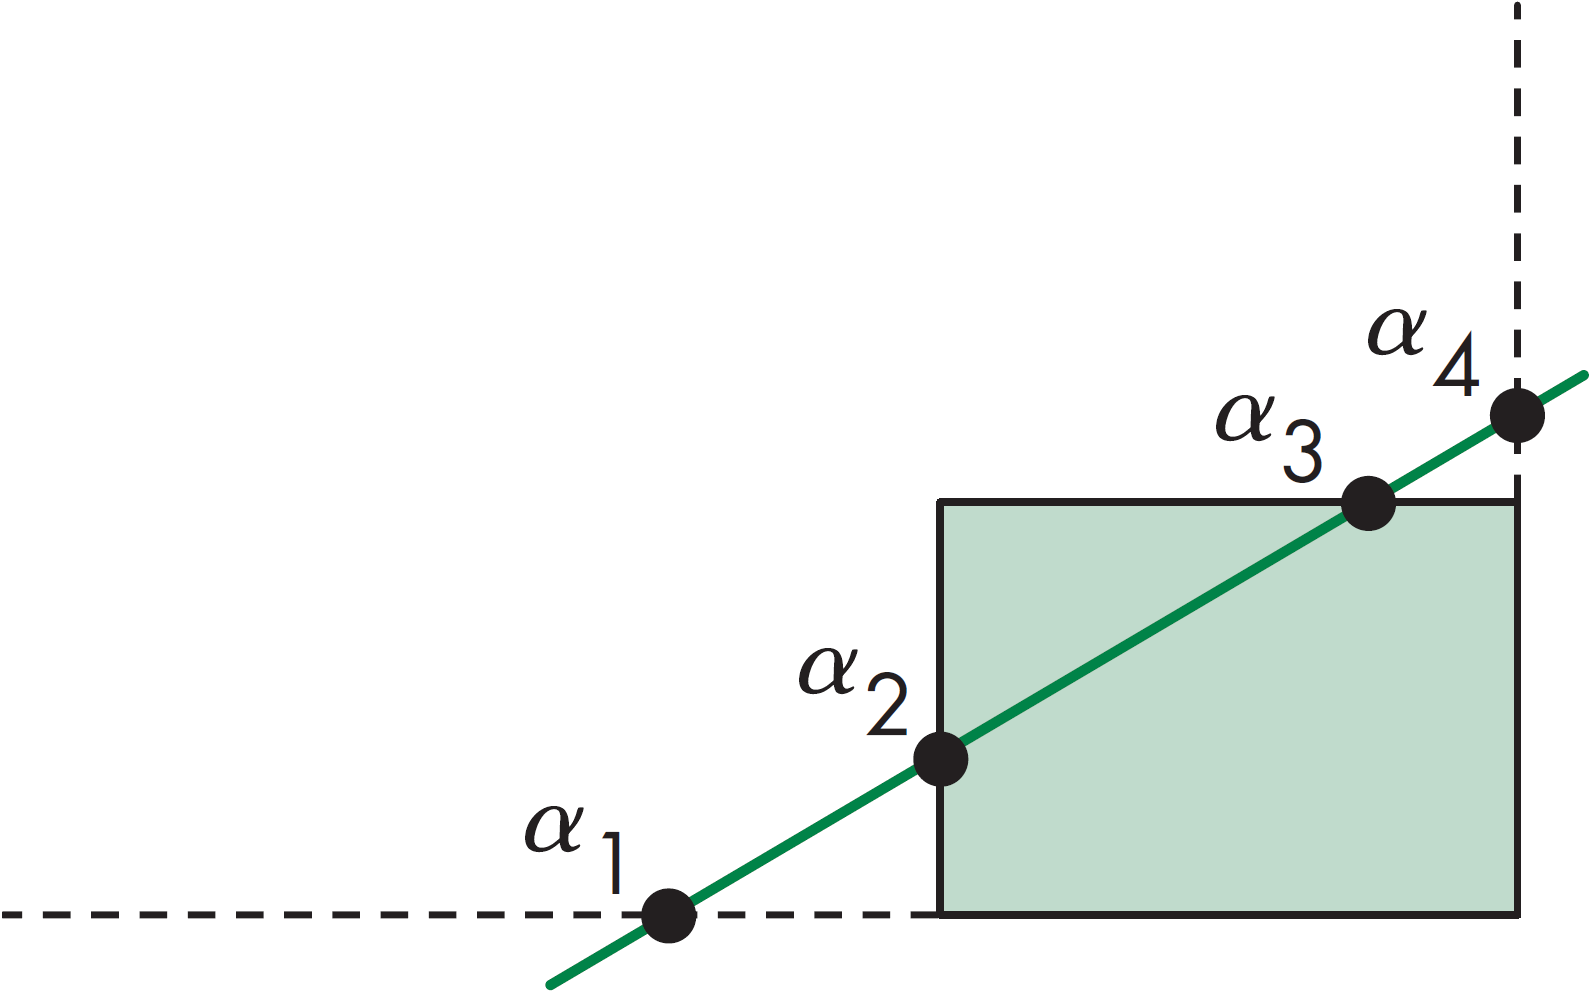
\includegraphics[width=\textwidth]{\main/images/chapter06/liang_a.png}
              \caption{Line Shown}
              \label{fig:liang_a}
            \end{subfigure}
            \begin{subfigure}{0.4\linewidth}
              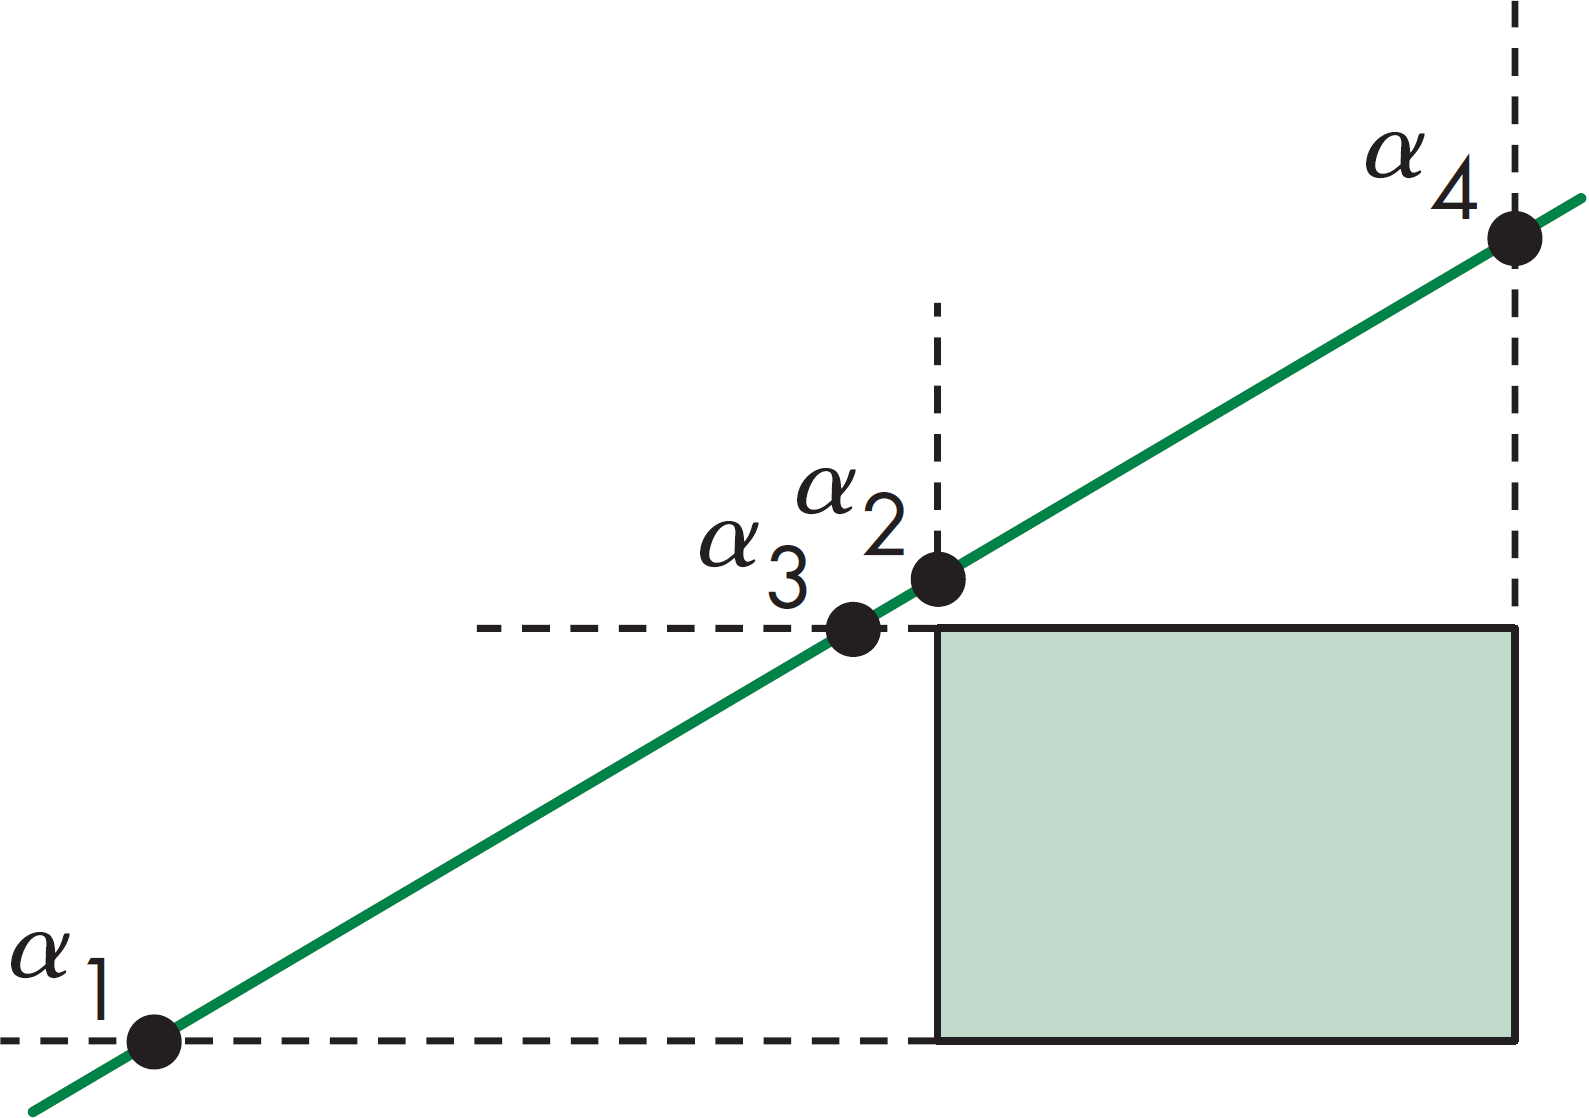
\includegraphics[width=\textwidth]{\main/images/chapter06/liang_b.png}
              \caption{Line Hidden}
              \label{fig:liang_b}
            \end{subfigure}
            \caption{Two cases of a parametric line and a clipping window}
          \end{center}

          In \autoref{fig:liang_a}, we can see that
          \begin{align*}
            1 > \alpha_4 > \alpha_3 > \alpha_2 > \alpha_1 > 0.
          \end{align*}
          This means all intersections are inside the original line segment, and the two innermost
          ($\alpha_2$~and~$\alpha_3$) determine the clipped segment.

          We can distinguish this case from the case in \autoref{fig:liang_b},
          which also has the four intersections between the endpoints of the line segment,
          by noting that the order for this case is
          \begin{align*}
            1 > \alpha_4 > \alpha_2 > \alpha_3 > \alpha_1 > 0.
          \end{align*}
          The line intersects both the top and the bottom of the extended window before it
          intersects either the left or the right; thus, the entire line segment must be
          rejected.
        \end{example}

        All decisions about clipping can be made without floating point division.
        Only if an intersection is needed (because a segment has to be shortened)
        is the division done.

        The efficiency of this approach, compared with Cohen-Sutherland, is that we avoid
        multiple shortenings of line segments and related re-executions of the clipping
        algorithm.

\end{document}
